% Options for packages loaded elsewhere
\PassOptionsToPackage{unicode}{hyperref}
\PassOptionsToPackage{hyphens}{url}
\PassOptionsToPackage{dvipsnames,svgnames,x11names}{xcolor}
%
\documentclass[
  letterpaper,
  DIV=11,
  numbers=noendperiod]{scrartcl}

\usepackage{amsmath,amssymb}
\usepackage{iftex}
\ifPDFTeX
  \usepackage[T1]{fontenc}
  \usepackage[utf8]{inputenc}
  \usepackage{textcomp} % provide euro and other symbols
\else % if luatex or xetex
  \usepackage{unicode-math}
  \defaultfontfeatures{Scale=MatchLowercase}
  \defaultfontfeatures[\rmfamily]{Ligatures=TeX,Scale=1}
\fi
\usepackage{lmodern}
\ifPDFTeX\else  
    % xetex/luatex font selection
\fi
% Use upquote if available, for straight quotes in verbatim environments
\IfFileExists{upquote.sty}{\usepackage{upquote}}{}
\IfFileExists{microtype.sty}{% use microtype if available
  \usepackage[]{microtype}
  \UseMicrotypeSet[protrusion]{basicmath} % disable protrusion for tt fonts
}{}
\makeatletter
\@ifundefined{KOMAClassName}{% if non-KOMA class
  \IfFileExists{parskip.sty}{%
    \usepackage{parskip}
  }{% else
    \setlength{\parindent}{0pt}
    \setlength{\parskip}{6pt plus 2pt minus 1pt}}
}{% if KOMA class
  \KOMAoptions{parskip=half}}
\makeatother
\usepackage{xcolor}
\setlength{\emergencystretch}{3em} % prevent overfull lines
\setcounter{secnumdepth}{-\maxdimen} % remove section numbering
% Make \paragraph and \subparagraph free-standing
\ifx\paragraph\undefined\else
  \let\oldparagraph\paragraph
  \renewcommand{\paragraph}[1]{\oldparagraph{#1}\mbox{}}
\fi
\ifx\subparagraph\undefined\else
  \let\oldsubparagraph\subparagraph
  \renewcommand{\subparagraph}[1]{\oldsubparagraph{#1}\mbox{}}
\fi

\usepackage{color}
\usepackage{fancyvrb}
\newcommand{\VerbBar}{|}
\newcommand{\VERB}{\Verb[commandchars=\\\{\}]}
\DefineVerbatimEnvironment{Highlighting}{Verbatim}{commandchars=\\\{\}}
% Add ',fontsize=\small' for more characters per line
\usepackage{framed}
\definecolor{shadecolor}{RGB}{241,243,245}
\newenvironment{Shaded}{\begin{snugshade}}{\end{snugshade}}
\newcommand{\AlertTok}[1]{\textcolor[rgb]{0.68,0.00,0.00}{#1}}
\newcommand{\AnnotationTok}[1]{\textcolor[rgb]{0.37,0.37,0.37}{#1}}
\newcommand{\AttributeTok}[1]{\textcolor[rgb]{0.40,0.45,0.13}{#1}}
\newcommand{\BaseNTok}[1]{\textcolor[rgb]{0.68,0.00,0.00}{#1}}
\newcommand{\BuiltInTok}[1]{\textcolor[rgb]{0.00,0.23,0.31}{#1}}
\newcommand{\CharTok}[1]{\textcolor[rgb]{0.13,0.47,0.30}{#1}}
\newcommand{\CommentTok}[1]{\textcolor[rgb]{0.37,0.37,0.37}{#1}}
\newcommand{\CommentVarTok}[1]{\textcolor[rgb]{0.37,0.37,0.37}{\textit{#1}}}
\newcommand{\ConstantTok}[1]{\textcolor[rgb]{0.56,0.35,0.01}{#1}}
\newcommand{\ControlFlowTok}[1]{\textcolor[rgb]{0.00,0.23,0.31}{#1}}
\newcommand{\DataTypeTok}[1]{\textcolor[rgb]{0.68,0.00,0.00}{#1}}
\newcommand{\DecValTok}[1]{\textcolor[rgb]{0.68,0.00,0.00}{#1}}
\newcommand{\DocumentationTok}[1]{\textcolor[rgb]{0.37,0.37,0.37}{\textit{#1}}}
\newcommand{\ErrorTok}[1]{\textcolor[rgb]{0.68,0.00,0.00}{#1}}
\newcommand{\ExtensionTok}[1]{\textcolor[rgb]{0.00,0.23,0.31}{#1}}
\newcommand{\FloatTok}[1]{\textcolor[rgb]{0.68,0.00,0.00}{#1}}
\newcommand{\FunctionTok}[1]{\textcolor[rgb]{0.28,0.35,0.67}{#1}}
\newcommand{\ImportTok}[1]{\textcolor[rgb]{0.00,0.46,0.62}{#1}}
\newcommand{\InformationTok}[1]{\textcolor[rgb]{0.37,0.37,0.37}{#1}}
\newcommand{\KeywordTok}[1]{\textcolor[rgb]{0.00,0.23,0.31}{#1}}
\newcommand{\NormalTok}[1]{\textcolor[rgb]{0.00,0.23,0.31}{#1}}
\newcommand{\OperatorTok}[1]{\textcolor[rgb]{0.37,0.37,0.37}{#1}}
\newcommand{\OtherTok}[1]{\textcolor[rgb]{0.00,0.23,0.31}{#1}}
\newcommand{\PreprocessorTok}[1]{\textcolor[rgb]{0.68,0.00,0.00}{#1}}
\newcommand{\RegionMarkerTok}[1]{\textcolor[rgb]{0.00,0.23,0.31}{#1}}
\newcommand{\SpecialCharTok}[1]{\textcolor[rgb]{0.37,0.37,0.37}{#1}}
\newcommand{\SpecialStringTok}[1]{\textcolor[rgb]{0.13,0.47,0.30}{#1}}
\newcommand{\StringTok}[1]{\textcolor[rgb]{0.13,0.47,0.30}{#1}}
\newcommand{\VariableTok}[1]{\textcolor[rgb]{0.07,0.07,0.07}{#1}}
\newcommand{\VerbatimStringTok}[1]{\textcolor[rgb]{0.13,0.47,0.30}{#1}}
\newcommand{\WarningTok}[1]{\textcolor[rgb]{0.37,0.37,0.37}{\textit{#1}}}

\providecommand{\tightlist}{%
  \setlength{\itemsep}{0pt}\setlength{\parskip}{0pt}}\usepackage{longtable,booktabs,array}
\usepackage{calc} % for calculating minipage widths
% Correct order of tables after \paragraph or \subparagraph
\usepackage{etoolbox}
\makeatletter
\patchcmd\longtable{\par}{\if@noskipsec\mbox{}\fi\par}{}{}
\makeatother
% Allow footnotes in longtable head/foot
\IfFileExists{footnotehyper.sty}{\usepackage{footnotehyper}}{\usepackage{footnote}}
\makesavenoteenv{longtable}
\usepackage{graphicx}
\makeatletter
\def\maxwidth{\ifdim\Gin@nat@width>\linewidth\linewidth\else\Gin@nat@width\fi}
\def\maxheight{\ifdim\Gin@nat@height>\textheight\textheight\else\Gin@nat@height\fi}
\makeatother
% Scale images if necessary, so that they will not overflow the page
% margins by default, and it is still possible to overwrite the defaults
% using explicit options in \includegraphics[width, height, ...]{}
\setkeys{Gin}{width=\maxwidth,height=\maxheight,keepaspectratio}
% Set default figure placement to htbp
\makeatletter
\def\fps@figure{htbp}
\makeatother

\usepackage{booktabs}
\usepackage{longtable}
\usepackage{array}
\usepackage{multirow}
\usepackage{wrapfig}
\usepackage{float}
\usepackage{colortbl}
\usepackage{pdflscape}
\usepackage{tabu}
\usepackage{threeparttable}
\usepackage{threeparttablex}
\usepackage[normalem]{ulem}
\usepackage{makecell}
\usepackage{xcolor}
\KOMAoption{captions}{tableheading}
\makeatletter
\@ifpackageloaded{caption}{}{\usepackage{caption}}
\AtBeginDocument{%
\ifdefined\contentsname
  \renewcommand*\contentsname{Table of contents}
\else
  \newcommand\contentsname{Table of contents}
\fi
\ifdefined\listfigurename
  \renewcommand*\listfigurename{List of Figures}
\else
  \newcommand\listfigurename{List of Figures}
\fi
\ifdefined\listtablename
  \renewcommand*\listtablename{List of Tables}
\else
  \newcommand\listtablename{List of Tables}
\fi
\ifdefined\figurename
  \renewcommand*\figurename{Figure}
\else
  \newcommand\figurename{Figure}
\fi
\ifdefined\tablename
  \renewcommand*\tablename{Table}
\else
  \newcommand\tablename{Table}
\fi
}
\@ifpackageloaded{float}{}{\usepackage{float}}
\floatstyle{ruled}
\@ifundefined{c@chapter}{\newfloat{codelisting}{h}{lop}}{\newfloat{codelisting}{h}{lop}[chapter]}
\floatname{codelisting}{Listing}
\newcommand*\listoflistings{\listof{codelisting}{List of Listings}}
\makeatother
\makeatletter
\makeatother
\makeatletter
\@ifpackageloaded{caption}{}{\usepackage{caption}}
\@ifpackageloaded{subcaption}{}{\usepackage{subcaption}}
\makeatother
\ifLuaTeX
  \usepackage{selnolig}  % disable illegal ligatures
\fi
\usepackage{bookmark}

\IfFileExists{xurl.sty}{\usepackage{xurl}}{} % add URL line breaks if available
\urlstyle{same} % disable monospaced font for URLs
\hypersetup{
  pdftitle={Module 1 Script v2},
  colorlinks=true,
  linkcolor={blue},
  filecolor={Maroon},
  citecolor={Blue},
  urlcolor={Blue},
  pdfcreator={LaTeX via pandoc}}

\title{Module 1 Script v2}
\author{}
\date{}

\begin{document}
\maketitle

html: code-fold: true

\subsection{A Brief Analysis of Well-Being Data from U.S. Antarctic
Research Outpost 31 - Post Re-Opening
2024}\label{a-brief-analysis-of-well-being-data-from-u.s.-antarctic-research-outpost-31---post-re-opening-2024}

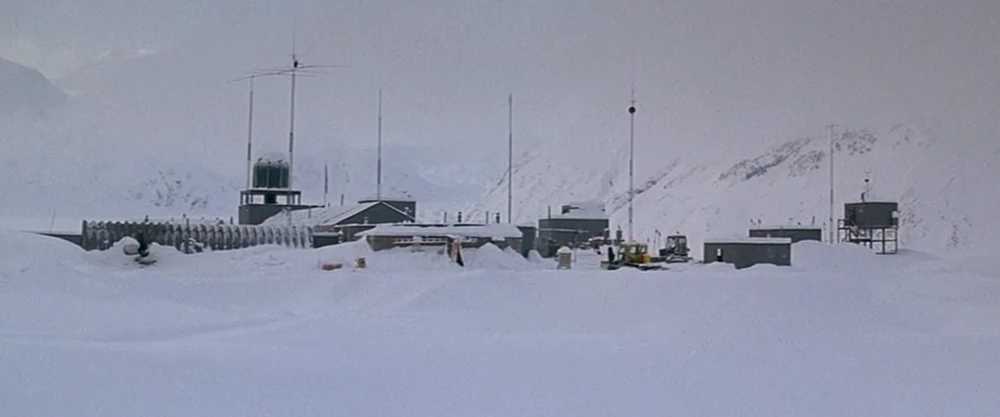
\includegraphics{images/U.S._Outpost_31_-_Profile.png}

We finally received the updated data on our study on the well-being of
scientists at our Antarctic Research Outpost 31\ldots{} which recently
re-opened for operations 41 years after the mysterious disaster of 1982
wherein occupant except for two survivors were mysteriously killed in
what looked like a gas leak\ldots or maybe the MRE's we shipped were
expired\ldots it doesn't matter! Science must continue! Surprisingly one
of the survivors, RJ MacReady agreed to serve as the field data monitor
for this project.

\includegraphics{images/the-thing-1.avif}

We sent 50 suckers\ldots I mean brave souls, men and women both, to
reopen the Outpost and spent months collecting self reported data on a
variety of metrics we think are related to well-being in harsh
environments. Before we dive in, just a note: this is a small sample
size, we may find that a lot of our descriptive values have very little
deviation and point toward many of our variable being considered
``normal''\ldots but we have to be careful with these assumptions and
actually visualize our data to confirm this suspicion. Let's dive in!

\begin{Shaded}
\begin{Highlighting}[]
\CommentTok{\# Load Packages and Dataset}

\FunctionTok{library}\NormalTok{(psych)}
\FunctionTok{library}\NormalTok{(tidyverse)}
\end{Highlighting}
\end{Shaded}

\begin{verbatim}
-- Attaching core tidyverse packages ------------------------ tidyverse 2.0.0 --
v dplyr     1.1.4     v readr     2.1.5
v forcats   1.0.0     v stringr   1.5.1
v ggplot2   3.5.0     v tibble    3.2.1
v lubridate 1.9.3     v tidyr     1.3.1
v purrr     1.0.2     
-- Conflicts ------------------------------------------ tidyverse_conflicts() --
x ggplot2::%+%()   masks psych::%+%()
x ggplot2::alpha() masks psych::alpha()
x dplyr::filter()  masks stats::filter()
x dplyr::lag()     masks stats::lag()
i Use the conflicted package (<http://conflicted.r-lib.org/>) to force all conflicts to become errors
\end{verbatim}

\begin{Shaded}
\begin{Highlighting}[]
\FunctionTok{library}\NormalTok{(kableExtra)}
\end{Highlighting}
\end{Shaded}

\begin{verbatim}

Attaching package: 'kableExtra'

The following object is masked from 'package:dplyr':

    group_rows
\end{verbatim}

\begin{Shaded}
\begin{Highlighting}[]
\FunctionTok{library}\NormalTok{(ggridges)}
\FunctionTok{library}\NormalTok{(reshape2)}
\end{Highlighting}
\end{Shaded}

\begin{verbatim}

Attaching package: 'reshape2'

The following object is masked from 'package:tidyr':

    smiths
\end{verbatim}

\begin{Shaded}
\begin{Highlighting}[]
\NormalTok{df }\OtherTok{\textless{}{-}} \FunctionTok{read.csv}\NormalTok{(}\StringTok{"mod1.csv"}\NormalTok{)}
\end{Highlighting}
\end{Shaded}

\subsubsection{Observing the whole data
set}\label{observing-the-whole-data-set}

\begin{table}
\centering
\begin{tabular}[t]{l|r|r|r|r|r|r|r|r|r|r|r|r|r}
\hline
  & vars & n & mean & sd & median & trimmed & mad & min & max & range & skew & kurtosis & se\\
\hline
x1 & 1 & 50 & 0.0181080 & 0.7695948 & -0.1175425 & -0.0385125 & 0.8966687 & -1.038504 & 1.934563 & 2.973067 & 0.5082616 & -0.6441462 & 0.1088371\\
\hline
x2 & 2 & 50 & -0.0266266 & 0.7772361 & -0.1097358 & -0.0527651 & 0.8519142 & -1.385028 & 1.788916 & 3.173945 & 0.2062904 & -0.8077550 & 0.1099178\\
\hline
x3 & 3 & 50 & -0.0778442 & 0.7697878 & 0.0267834 & -0.0917865 & 0.9536180 & -1.430250 & 1.486698 & 2.916948 & 0.1470770 & -0.9482259 & 0.1088644\\
\hline
x4 & 4 & 50 & 0.1126985 & 0.7531142 & 0.2082776 & 0.1115210 & 0.5747207 & -1.526286 & 2.302391 & 3.828677 & 0.0752375 & 0.3711921 & 0.1065064\\
\hline
x5 & 5 & 50 & 0.0428410 & 0.7391254 & 0.0287931 & 0.0523095 & 0.8074606 & -1.708452 & 1.525088 & 3.233540 & -0.0970308 & -0.6050263 & 0.1045281\\
\hline
x6 & 6 & 50 & 0.0883565 & 0.7290995 & 0.0657845 & 0.0627313 & 0.7918899 & -1.482324 & 1.929189 & 3.411514 & 0.2480144 & -0.4273610 & 0.1031102\\
\hline
x7 & 7 & 50 & 0.0051591 & 0.6827241 & -0.0320769 & -0.0079656 & 0.7399854 & -1.178929 & 1.562697 & 2.741626 & 0.1778498 & -0.8244356 & 0.0965518\\
\hline
x8 & 8 & 50 & -0.0355454 & 0.6456919 & 0.0901859 & -0.0086301 & 0.7667231 & -1.435320 & 1.241873 & 2.677193 & -0.2829005 & -0.9115552 & 0.0913146\\
\hline
x9 & 9 & 50 & -0.0685567 & 0.8152215 & -0.0379734 & -0.1065734 & 0.9954745 & -1.556594 & 1.805193 & 3.361788 & 0.3186261 & -0.8222238 & 0.1152897\\
\hline
x10 & 10 & 50 & 0.0730629 & 0.7774751 & 0.2515162 & 0.0903750 & 1.0427794 & -1.808745 & 1.375211 & 3.183956 & -0.2367742 & -1.0518567 & 0.1099516\\
\hline
y & 11 & 50 & 0.0155731 & 0.6931878 & 0.1166201 & 0.0133267 & 0.8215418 & -1.586415 & 1.419483 & 3.005897 & -0.0415111 & -0.6472254 & 0.0980316\\
\hline
\end{tabular}
\end{table}

\begin{Shaded}
\begin{Highlighting}[]
\CommentTok{\# Melt the data to long format}
\NormalTok{df\_long }\OtherTok{\textless{}{-}} \FunctionTok{melt}\NormalTok{(df)}
\end{Highlighting}
\end{Shaded}

\begin{verbatim}
Using sex as id variables
\end{verbatim}

\begin{Shaded}
\begin{Highlighting}[]
\CommentTok{\# Plot histograms using ggplot and facet\_wrap}
\CommentTok{\# Used Sturges\textquotesingle{} Rule k=⌈log2(n)+1⌉ to calculate bins}
\FunctionTok{ggplot}\NormalTok{(df\_long, }\FunctionTok{aes}\NormalTok{(}\AttributeTok{x =}\NormalTok{ value)) }\SpecialCharTok{+}
  \FunctionTok{geom\_histogram}\NormalTok{(}\AttributeTok{bins =} \DecValTok{7}\NormalTok{, }\AttributeTok{fill =} \StringTok{"dodgerblue"}\NormalTok{, }\AttributeTok{color =} \StringTok{"white"}\NormalTok{) }\SpecialCharTok{+}
  \FunctionTok{facet\_wrap}\NormalTok{(}\SpecialCharTok{\textasciitilde{}}\NormalTok{ variable, }\AttributeTok{scales =} \StringTok{"free"}\NormalTok{) }\SpecialCharTok{+}  \CommentTok{\# Create one histogram for each variable}
  \FunctionTok{labs}\NormalTok{(}\AttributeTok{title =} \StringTok{"Histograms for Each Variable"}\NormalTok{,}
       \AttributeTok{x =} \StringTok{"Value"}\NormalTok{, }
       \AttributeTok{y =} \StringTok{"Freq"}\NormalTok{) }\SpecialCharTok{+}
  \FunctionTok{theme\_minimal}\NormalTok{()}
\end{Highlighting}
\end{Shaded}

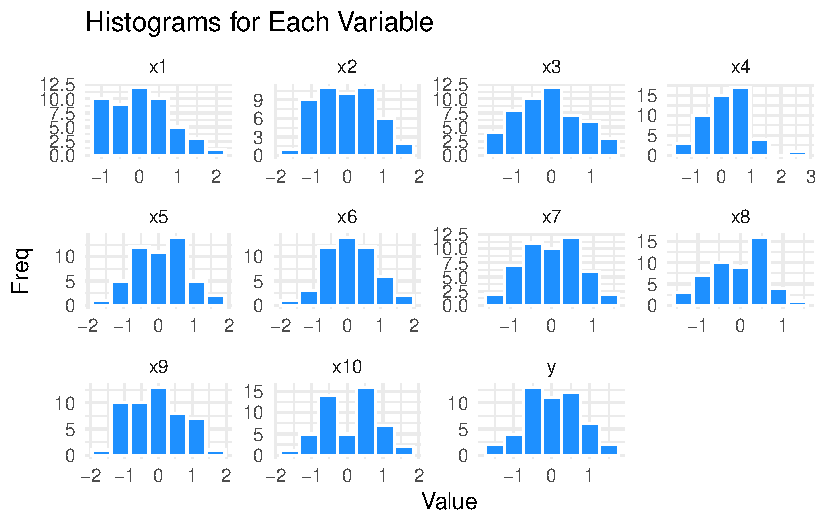
\includegraphics{Module-1-Script-v2_files/figure-pdf/unnamed-chunk-3-1.pdf}

Based on this overview, it looks like the data was already scaled before
it was delivered for analysis\ldots Johnson! Remind MacReady not to mess
with the data before it gets to the lab! Jesus Christ what do I pay you
all for?

Anyway, we can't exactly assume that either, so whenever we decide to
compare any of these variable together, we'll use a Z
transform\ldots more on that later. Onto the exploratory data analysis:

X4 and X1 are looking interesting\ldots X4 appears to have an outlier
(remember what I said about the small sample size?) so we'll have to
zoom in there to see what's going on. And X1, looks like a positive
skew\ldots wonder how strongly that's actually going to relate to Y.
Let's focus on those two for now.

\begin{Shaded}
\begin{Highlighting}[]
\FunctionTok{ggplot}\NormalTok{(df, }\FunctionTok{aes}\NormalTok{(}\AttributeTok{x=}\NormalTok{x4)) }\SpecialCharTok{+} \FunctionTok{geom\_histogram}\NormalTok{(}\AttributeTok{binwidth=}\FloatTok{0.5}\NormalTok{, }\AttributeTok{fill=}\StringTok{"dodgerblue"}\NormalTok{, }\AttributeTok{color=}\StringTok{"white"}\NormalTok{, }\FunctionTok{aes}\NormalTok{(}\AttributeTok{y=}\NormalTok{..density..)) }\SpecialCharTok{+} \FunctionTok{geom\_density}\NormalTok{(}\AttributeTok{alpha=}\NormalTok{.}\DecValTok{4}\NormalTok{, }\AttributeTok{fill=}\StringTok{"firebrick"}\NormalTok{, }\AttributeTok{color=}\StringTok{"NA"}\NormalTok{) }\SpecialCharTok{+} \FunctionTok{stat\_function}\NormalTok{(}\AttributeTok{fun=}\NormalTok{dnorm, }\AttributeTok{args=}\FunctionTok{list}\NormalTok{(}\AttributeTok{mean=}\FunctionTok{mean}\NormalTok{(df}\SpecialCharTok{$}\NormalTok{x4), }\AttributeTok{sd=}\FunctionTok{sd}\NormalTok{(df}\SpecialCharTok{$}\NormalTok{x4)), }\AttributeTok{color=}\StringTok{"black"}\NormalTok{, }\AttributeTok{size=}\DecValTok{1}\NormalTok{) }\SpecialCharTok{+} \FunctionTok{theme\_minimal}\NormalTok{()}
\end{Highlighting}
\end{Shaded}

\begin{verbatim}
Warning: Using `size` aesthetic for lines was deprecated in ggplot2 3.4.0.
i Please use `linewidth` instead.
\end{verbatim}

\begin{verbatim}
Warning: The dot-dot notation (`..density..`) was deprecated in ggplot2 3.4.0.
i Please use `after_stat(density)` instead.
\end{verbatim}

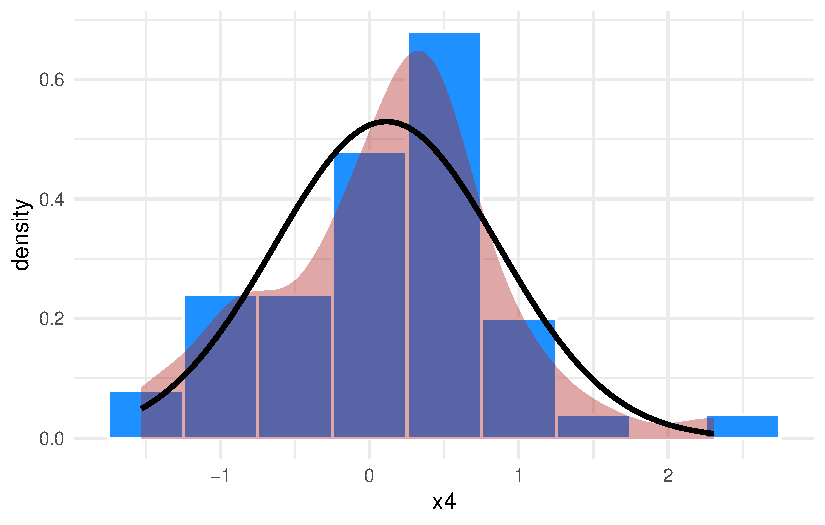
\includegraphics{Module-1-Script-v2_files/figure-pdf/unnamed-chunk-4-1.pdf}

\begin{Shaded}
\begin{Highlighting}[]
\FunctionTok{ggplot}\NormalTok{(df, }\FunctionTok{aes}\NormalTok{(}\AttributeTok{x=}\NormalTok{x9)) }\SpecialCharTok{+} \FunctionTok{geom\_histogram}\NormalTok{(}\AttributeTok{binwidth=}\FloatTok{0.5}\NormalTok{, }\AttributeTok{fill=}\StringTok{"dodgerblue"}\NormalTok{, }\AttributeTok{color=}\StringTok{"white"}\NormalTok{, }\FunctionTok{aes}\NormalTok{(}\AttributeTok{y=}\NormalTok{..density..)) }\SpecialCharTok{+} \FunctionTok{geom\_density}\NormalTok{(}\AttributeTok{alpha=}\NormalTok{.}\DecValTok{4}\NormalTok{, }\AttributeTok{fill=}\StringTok{"firebrick"}\NormalTok{, }\AttributeTok{color=}\StringTok{"NA"}\NormalTok{) }\SpecialCharTok{+} \FunctionTok{stat\_function}\NormalTok{(}\AttributeTok{fun=}\NormalTok{dnorm, }\AttributeTok{args=}\FunctionTok{list}\NormalTok{(}\AttributeTok{mean=}\FunctionTok{mean}\NormalTok{(df}\SpecialCharTok{$}\NormalTok{x4), }\AttributeTok{sd=}\FunctionTok{sd}\NormalTok{(df}\SpecialCharTok{$}\NormalTok{x4)), }\AttributeTok{color=}\StringTok{"black"}\NormalTok{, }\AttributeTok{size=}\DecValTok{1}\NormalTok{) }\SpecialCharTok{+} \FunctionTok{theme\_minimal}\NormalTok{()}
\end{Highlighting}
\end{Shaded}

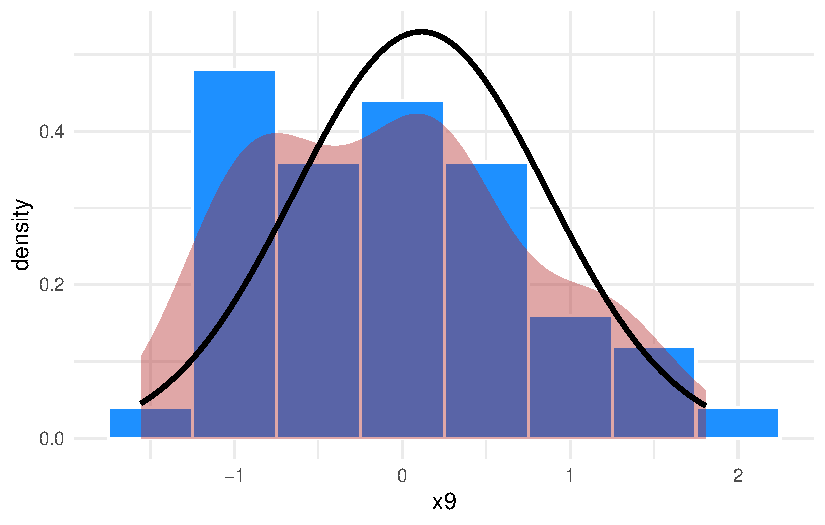
\includegraphics{Module-1-Script-v2_files/figure-pdf/unnamed-chunk-5-1.pdf}

\subsubsection{Digging into specific
variables}\label{digging-into-specific-variables}

\begin{Shaded}
\begin{Highlighting}[]
\CommentTok{\# Generate histograms and overlay density plots, normal dist, and SD\textquotesingle{}s, and lop off outliers [explain why]}

\NormalTok{x4z }\OtherTok{\textless{}{-}} \FunctionTok{scale}\NormalTok{(df}\SpecialCharTok{$}\NormalTok{x4)}
\NormalTok{x9z }\OtherTok{\textless{}{-}} \FunctionTok{scale}\NormalTok{(df}\SpecialCharTok{$}\NormalTok{x9)}

\CommentTok{\# fix the axes so that the density and histogram agree on the y axis}
\FunctionTok{ggplot}\NormalTok{(df, }\FunctionTok{aes}\NormalTok{(}\AttributeTok{x=}\NormalTok{x4)) }\SpecialCharTok{+} 
  \FunctionTok{geom\_histogram}\NormalTok{(}\AttributeTok{binwidth=}\FloatTok{0.5}\NormalTok{, }\AttributeTok{fill=}\StringTok{"dodgerblue"}\NormalTok{, }\AttributeTok{color=}\StringTok{"white"}\NormalTok{, }\FunctionTok{aes}\NormalTok{(}\AttributeTok{y=}\NormalTok{..density..)) }\SpecialCharTok{+} 
  \FunctionTok{geom\_density}\NormalTok{(}\AttributeTok{alpha=}\NormalTok{.}\DecValTok{2}\NormalTok{, }\AttributeTok{fill=}\StringTok{"red"}\NormalTok{) }\SpecialCharTok{+}
  \FunctionTok{theme\_minimal}\NormalTok{()}
\end{Highlighting}
\end{Shaded}

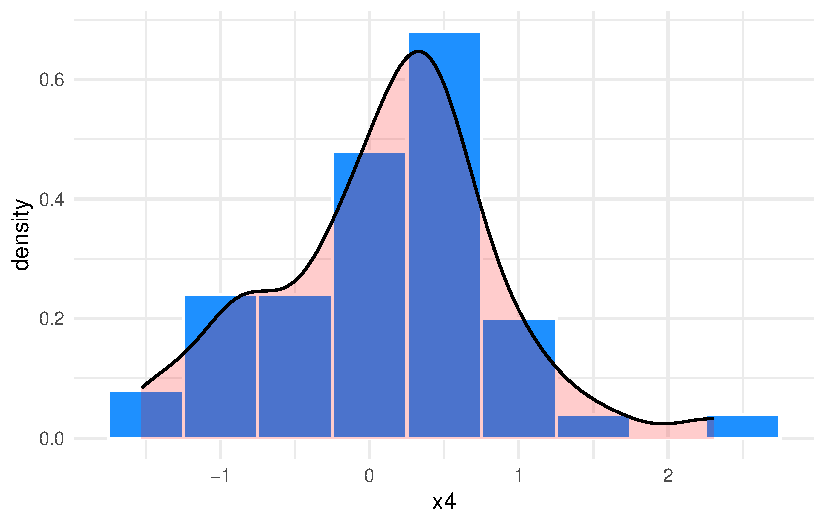
\includegraphics{Module-1-Script-v2_files/figure-pdf/unnamed-chunk-6-1.pdf}

\begin{Shaded}
\begin{Highlighting}[]
\FunctionTok{ggplot}\NormalTok{(df, }\FunctionTok{aes}\NormalTok{(}\AttributeTok{x=}\NormalTok{x9)) }\SpecialCharTok{+} 
  \FunctionTok{geom\_histogram}\NormalTok{(}\AttributeTok{binwidth=}\FloatTok{0.5}\NormalTok{, }\AttributeTok{fill=}\StringTok{"dodgerblue"}\NormalTok{, }\AttributeTok{color=}\StringTok{"white"}\NormalTok{, }\FunctionTok{aes}\NormalTok{(}\AttributeTok{y=}\NormalTok{..density..)) }\SpecialCharTok{+} 
  \FunctionTok{geom\_density}\NormalTok{(}\AttributeTok{alpha=}\NormalTok{.}\DecValTok{2}\NormalTok{, }\AttributeTok{fill=}\StringTok{"red"}\NormalTok{) }\SpecialCharTok{+}
  \FunctionTok{theme\_minimal}\NormalTok{()}
\end{Highlighting}
\end{Shaded}

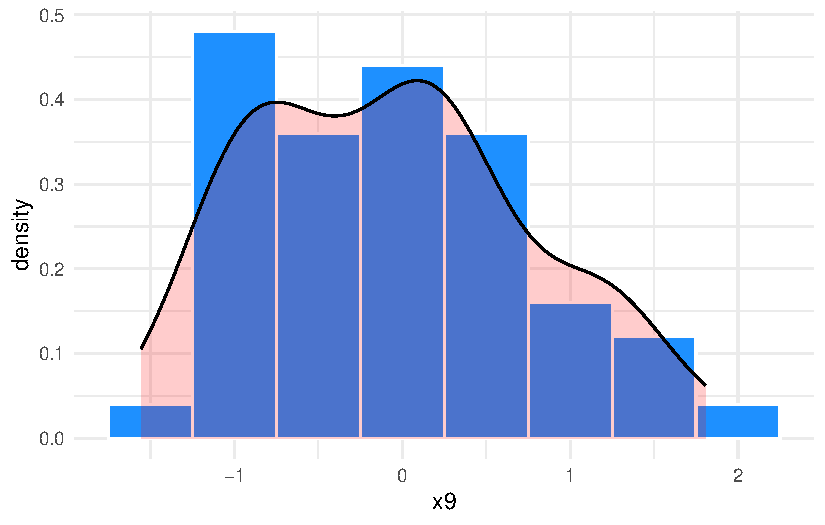
\includegraphics{Module-1-Script-v2_files/figure-pdf/unnamed-chunk-7-1.pdf}

\begin{Shaded}
\begin{Highlighting}[]
\FunctionTok{ggplot}\NormalTok{(df, }\FunctionTok{aes}\NormalTok{(}\AttributeTok{x =}\NormalTok{ x4z)) }\SpecialCharTok{+} 
  \FunctionTok{geom\_histogram}\NormalTok{(}\AttributeTok{binwidth =} \FloatTok{0.5}\NormalTok{, }\AttributeTok{fill =} \StringTok{"dodgerblue"}\NormalTok{, }\AttributeTok{color =} \StringTok{"white"}\NormalTok{, }\FunctionTok{aes}\NormalTok{(}\AttributeTok{y =}\NormalTok{ ..density..)) }\SpecialCharTok{+} 
  \FunctionTok{geom\_density}\NormalTok{(}\AttributeTok{alpha =} \FloatTok{0.2}\NormalTok{, }\AttributeTok{fill =} \StringTok{"red"}\NormalTok{, }\AttributeTok{color=}\StringTok{"white"}\NormalTok{) }\SpecialCharTok{+}
  \FunctionTok{facet\_wrap}\NormalTok{(}\SpecialCharTok{\textasciitilde{}}\NormalTok{ sex) }\SpecialCharTok{+}  \CommentTok{\# Facet the plot by the sex variable}
  \FunctionTok{theme\_minimal}\NormalTok{() }\SpecialCharTok{+}
  \FunctionTok{labs}\NormalTok{(}\AttributeTok{title =} \StringTok{"Histogram and Density of x4 Faceted by Sex"}\NormalTok{, }\AttributeTok{x =} \StringTok{"x4"}\NormalTok{, }\AttributeTok{y =} \StringTok{"Density"}\NormalTok{)}
\end{Highlighting}
\end{Shaded}

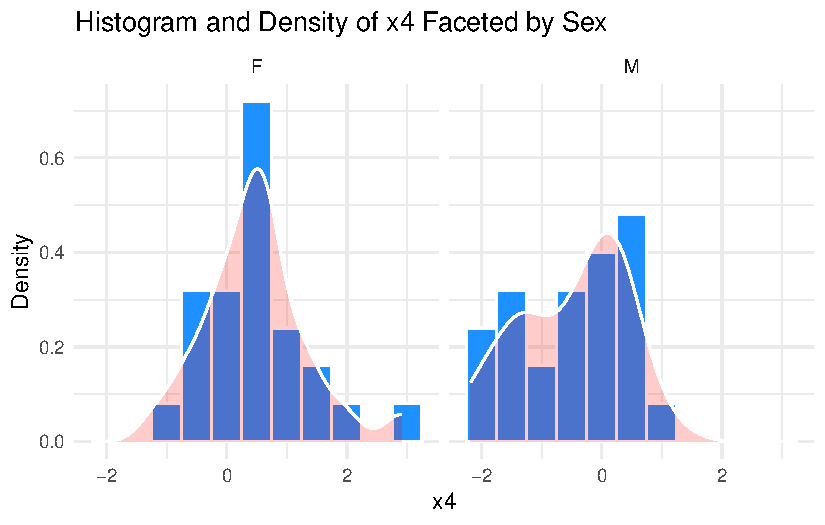
\includegraphics{Module-1-Script-v2_files/figure-pdf/unnamed-chunk-8-1.pdf}

\subsubsection{Comparing Variables}\label{comparing-variables}

\begin{Shaded}
\begin{Highlighting}[]
\CommentTok{\# Scale and compare variables}

\FunctionTok{ggplot}\NormalTok{(df, }\FunctionTok{aes}\NormalTok{(}\AttributeTok{x=}\NormalTok{x4z, }\AttributeTok{y=}\NormalTok{x9z)) }\SpecialCharTok{+}
  \FunctionTok{geom\_point}\NormalTok{(}\AttributeTok{size=}\DecValTok{3}\NormalTok{, }\AttributeTok{shape=}\DecValTok{16}\NormalTok{) }\SpecialCharTok{+}
  \FunctionTok{geom\_smooth}\NormalTok{(}\AttributeTok{method=}\StringTok{"lm"}\NormalTok{, }\AttributeTok{se=}\ConstantTok{TRUE}\NormalTok{) }\SpecialCharTok{+}
  \FunctionTok{theme\_minimal}\NormalTok{()}
\end{Highlighting}
\end{Shaded}

\begin{verbatim}
`geom_smooth()` using formula = 'y ~ x'
\end{verbatim}

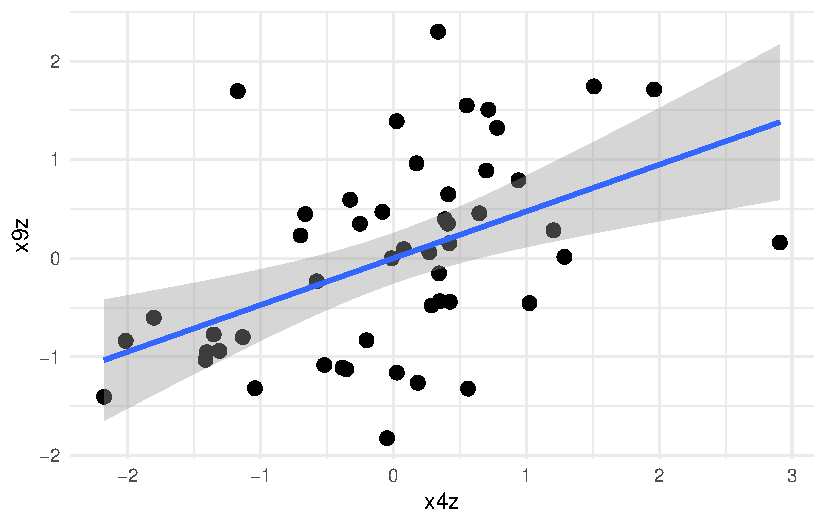
\includegraphics{Module-1-Script-v2_files/figure-pdf/unnamed-chunk-9-1.pdf}

\begin{Shaded}
\begin{Highlighting}[]
\CommentTok{\# Compare variables and generate a linear fit plot to discuss visual correlation}
\end{Highlighting}
\end{Shaded}




\end{document}
